\documentclass[50pt]{article}
\RequirePackage{pdfpages}
\renewcommand{\baselinestretch}{1.4}
\RequirePackage{amsthm,amssymb,amsmath,graphicx}
\RequirePackage{color}
\RequirePackage[top=2cm, bottom=2cm, left=2.5cm, right=3cm]{geometry}
\RequirePackage[pagebackref=false,colorlinks,linkcolor=blue,citecolor=magenta]{hyperref}
\RequirePackage{xepersian}
\RequirePackage{MnSymbol}
\RequirePackage{graphicx}
\newcommand{\wid}{1.8in}
\newtheorem{theorem}{Theorem}
\newcommand{\hl}{
\begin{center}
\line(1,0){450}
\end{center}}
\newenvironment{amatrix}[1]{%
\left[\begin{array}{@{}*{#1}{c}|c@{}}
}{%
\end{array}\right]
}
\settextfont{B Nazanin}
\setlatintextfont{Times New Roman}

\begin{document}
\setLTR 




\begin{RTL}
\Large{








\begin{center}
به نام خدا

پاسخ سوالات کوییز 1
\end{center}
\hl
\textbf{سوال 1) دوره تناوب سیگنال 
$x(t)=\delta(\sin t)$ را به دست آورید.}

پاسخ: از تعریف سیگنال متناوب، می توان گفت سیگنال پیوسته‌ی $x(t)$ با دوره‌ی تناوب $T$ متناوب است اگر وتنها اگر:
$$
x(t+T)=x(t)
$$
و به کمترین مقدار $T$ که رابطه‌ی بالا را برقرار سازد، دوره تناوب اساسی گفته می شود. تعریف مشابهی را برای سیگنال ها گسسته نیز می توان برقرار کرد. در این سوال، عنصر متناوب کننده‌ی سیگنال $x(t)$، تابع $\sin t$ است که با دوره‌ی اساسی $2\pi$ متناوب است؛ از طرفی:
$$
\sin (t+2\pi)=\sin t
$$
$$
\sin (t+\pi)=-\sin t
$$
چون $\delta(t)$ تابعی زوج است، می توان نوشت:
$$
\delta(\sin (t+2\pi))=\delta(\sin t)
$$
$$
\delta(\sin (t+\pi))=\delta(-\sin t)=\delta(\sin t)
$$
بنابراین 
\underline{دوره تناوب سیگنال $\delta(\sin t)$ برابر $\pi$ است.}
\hl
سوال 2) اگر $x(-2t+1)$ به صورت زیر باشد، مطلوب است 
$\int_{-1}^{0}x(t)dt$
\begin{center}
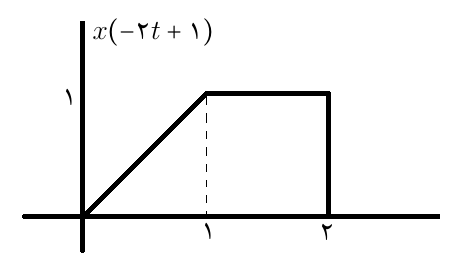
\includegraphics[width=65mm]{m5}
\end{center}

















}





\end{RTL}



\end{document}


